\documentclass[11pt,a4paper]{article}
\usepackage{jheppub}
\usepackage{physics}
\usepackage{tensor}
\usepackage{amsmath, bm}

\newcommand{\lagr}{\mathcal{L}}

\title{Reconstructing the connectivity of neuro-networks}
\author{Zihui Wang}
\affiliation{Department of Physics, New York University\\
New York, NY 10003\\
United States}

\emailAdd{zihui.wang@nyu.edu}
\abstract{A new method to reconstruct the connectivity of the neuro-network is proposed.}


\begin{document}
\maketitle
%\flushbottom

\section{Problem}
Consider a neuro-network of $N$ nodes modeled by the following coupled ODEs[1]
\begin{equation}
    \dot{x}_i = f(x_i) + \sum_{j=1}^N g_{ij}A_{ij}h(x_j-x_i)+\eta_i,
\end{equation}
where $x_i$ for $i=1,2,\cdots,N$ are the state variable for each node, and the time evolution $x_i(t)$ can be measured at $M$ times. The function $f$ denotes the intrinsic dynamics of the nodes and is identical for all $i$. The coefficients $g_{ij}$ measures the coupling strength between the $i$ and $j$th node. The matrix $A_{ij}$ is the connectivity matrix, with all the entries to be either $0$ or $1$ determining whether the $i$th and $j$th node are connected. Finally, $\eta_i$ is a Gaussian white noise with the statistics $\overline{\eta_i(t)\eta_j(t')}=\sigma^2\delta_{ij}\delta(t-t')$. The question of interest is to reconstruct the coefficient $g_{ij}A_{ij}$ given the form of the function $f$ and $h$, and $x_i(t)$ measured at $M$ time steps. The typical numbers are $N\sim100$ and $M\sim10^6$.

The existing method[2] has assumed various conditions, 1) the intrinsic dynamics $f(x_i)\approx0$ is negligible; 2) the coupling strength is uniform, $g_{ij}=g$; 3) the connectivity is bidirectional, i.e. the matrix $A_{ij}$ is symmetric and 4) the function $h(x_j-x_i)$ is linear.

\section{Proposed method}
We propose a simple method in which the aforementioned conditions can be relaxed. First, from the measured data $x_i(t)$ obtain $v_i(t)=\dot{x}_i(t)$, and regard it as a distinct variable. 
Consider one node, say $x_1(t)$. We will determine $\alpha_{1j}=g_{1j}A_{1j}$ by least square fit, which minimizes
\begin{equation}
   D = \sum_{t}\left[ v_1(t)- \sum_j\beta_{1j}h(x_j(t)-x_1(t))\right]^2.
\end{equation}
where $\beta$ will be the estimate of $\alpha$. The minimization leads to
\begin{equation}
   \pdv{D}{\beta_{1k}} = -2\sum_{t}\left[v_1(t)- \sum_k\beta_{1k}h(x_k(t)-x_1(t))\right]h(x_j(t)-x_1(t))=0.
\end{equation}
Finally, we have
\begin{equation}
   \beta_{1j} = \sum_{i}\mathcal{M}_{ji}u_i,
\end{equation}
with
\begin{gather}
    \mathcal{M} = \left[\sum_t h(x_i(t)-x_1(t)) h(x_j(t)-x_1(t))\right]^{-1}, \\
    u_i = \sum_t v_1(t)  h(x_i(t)-x_1(t)).
\end{gather}
The essence of the method is inverting $(N-1)\times(N-1)$ matrices, which, for $N\sim100$, is not in principle difficult. 

\section{Toy model: two nodes}
\subsection{Linear and symmetric coupling}
Consider a toy model of two nodes with the dynamics
\begin{gather}
    \dot{x}_1 = \alpha (x_2-x_1) +\eta_1, \\
    \dot{x}_2 = \alpha (x_1-x_2) +\eta_2.
\end{gather}
The goal is to determine the value of $\alpha$ given $x_1(t)$ and $x_2(t)$ as function of time. Adding and subtracting the two ODEs decouple the dynamics into
\begin{gather}
    \dot{x} = \eta, \\
    \dot{y} = -2\alpha y + \xi.
\end{gather}
The center-of-mass is governed by a random walk with $\langle x^2(t)\rangle \sim t$ while the relative distance $y$ is subject to a noise-driven dynamics. 

\subsubsection{Numerical treatment}
Our strategy is to choose a value of $\alpha$ first, say, $\alpha = 1$. Otherwise, we would not be able to generate $y(t)$. We solve the stochastic ODE $\dot{y}(t) = -2\alpha y + \xi$ by the simple Euler-forward method, that is
\begin{equation}
    y(t+\Delta t) = y(t) + (-2\alpha y+\xi)\Delta t.
\end{equation}
Note that discretizing the gaussian white noise produces a normalization factor $\xi \rightarrow \xi/\sqrt{\Delta t}$. After obtaining $y(t)$, we extract the ``velocity'' by finite-differencing
\begin{equation}
    v(t) \equiv \frac{ y(t+\Delta t)-y(t)}{\Delta t}.
\end{equation}
Then we are able to use the least square fit for 
\begin{equation}
    v(t)=-2\beta y,
\end{equation}
which yields
\begin{equation}
    -2\beta = \frac{\expval{v(t)y(t)}}{\expval{y(t)y(t)}}.
\end{equation}

\subsubsection{Analytics}
The equation for $y$ can be analytically solved in terms of the Green's function,
\begin{equation}
   \dot{G}(t) + 2\alpha G(t) = \delta(t)
\end{equation}
leading to
\begin{equation}
   G(t) = e^{-2\alpha t} \qq{for} t>0.
\end{equation}
Hence,
\begin{equation}
   y(t) = y_h(t) + \int_0^t dt'\, e^{-2\alpha t'} \xi(t').
\end{equation}
This allows us to calculate
\begin{equation}
   \frac{\Delta \beta^2}{\alpha^2} = \frac{2}{M\Delta t}\alpha
   \label{eqn:analytic1}
\end{equation}
where $M$ is the number of time steps and $\Delta t$ the length of every time step. The uncertainty in $\beta$ is interestingly independent of the noise. The reason for this will become clear later.

Note that $\tau=1/2\alpha$ is the characteristic time scale. In numerical treatments it must be ensured that $\Delta t<< \tau$ and $M\Delta t >> \tau$. Otherwise the system is not stabilized and will depend sensitively on initial conditions.

\subsubsection{Results}
Figure~\ref{fig:1} shows the distribution of reconstructed value of $\beta$ from 1000 runs each with 1000 time steps. The statistics is $\beta=1.009\pm0.017$. To compare with the analytic formula Eq.~\ref{eqn:analytic1} we must set $M= 10^3\times10^3 = 10^6$ to set up the equivalency which can be guaranteed by the principle of statistical physics that ensemble average equals time average for system at thermal equilibrium. So that the analytic uncertainty is 0.014, in reasonable agreement with the root mean square deviation from statistics.

Figure~\ref{fig:2} shows the dependence of $\Delta \beta$ in the level of the noise $\sigma$. The value of $\Delta\beta$ hovers around 0.017 as $\sigma$ increments. This verifies the independence of $\Delta\beta$ in $\sigma$.

To understand this independence, we study the scatter of $v$ versus $y$. Figure~\ref{fig:3} shows the scatter of $v(t)$ and $y(t)$ for 1000 time steps, with the level of noise $\sigma=0.5$. In Figure~\ref{fig:4} the level of the noise is doubled, and as a result, both the range of $v$ and $y$ are double. Therefore, the overall effect of noise on $\beta$ cancels out. Qualitatively, we can understand this as follows: the noise makes the finite-differencing inaccurate, the larger the noise the larger the inaccuracy. On the other hand, a large noise drives the node moves farther which increases the range of $y$. The two effects balance the uncertainty in $\beta$.

There is also a debate on whether the scatter plot leads to a legitimate linear fit line (which are shown in the figure as the red line). The point is that the fitting in this case is not to be understood as the fitting in the usual case. Our purpose is to obtain the connectivity (which is done by performing the fit), not to establish a linear relation between $v$ and $y$. 

Also it was questioned on whether these scatter points are correlated. Although it does not seem to exhibit any correlation on the figure, theoretically the two-point (strictly speaking, two-time) correlation
\begin{equation}
    \lim_{t_1\rightarrow\infty}\expval{y(t_1)y(t_2)} = \frac{\sigma^2}{2\alpha} (1-e^{-2\alpha t_2})
\end{equation}
is non-vanishing for $t_2>0$. 

\subsection{Linear and asymmetric coupling}
Next we consider a slightly more general situation where the coupling is asymmetric between the two nodes,
\begin{gather}
    \dot{x}_1 = \alpha_1 (x_2-x_1) +\eta_1, \\
    \dot{x}_2 = \alpha_2 (x_1-x_2) +\eta_2.
\end{gather}
Figure~\ref{fig:5} shows the reconstructed connectivity for $\alpha_1=1$ and $\alpha_2=2$. The distribution is from 1000 thousand runs. Statistics is $\beta_1=1.035 \pm 0.041$ and $\beta_2=1.982 \pm 0.065$.

\subsection{Nonlinear coupling}
As a last test for the two-node system, we consider the sinusoidal coupling 
\begin{gather}
    \dot{x}_1 = \alpha_1 \sin(x_2-x_1) +\eta_1, \\
    \dot{x}_2 = \alpha_2 \sin(x_1-x_2) +\eta_2.
\end{gather}
Again we have set $\alpha_1=1$ and $\alpha_2=2$. The reconstructed values are $\beta_1=1.011 \pm 0.038$ and $\beta_2=2.015 \pm 0.017$. The distribution is shown in Figure~\ref{fig:6}.

\section{Realistic model: multiple nodes}
In this section we consider system with $N\geq 3$ nodes. For simplicity, we will stick to the linear coupling case, which of course we could have relaxed. The dynamics is governed by the coupled ODEs
\begin{equation}
    \dot{x}_i = \sum_{j=1}^N \alpha_{ij} (x_j-x_i)+\eta_i,
\end{equation}
which can be rewritten as
\begin{equation}
    \dot{\vec{x}} = -L\vec{x} + \vec{\eta},
\end{equation}
where $\vec{x}=(x_1,x_2,...,x_N)$, $\vec{\eta}=(\eta_1,\eta_2,...,\eta_N)$ and the matrix $L$ is given by
\begin{equation}
    L_{ij} = \left(\sum_{j}\alpha_{ij}\right)\delta_{ij} - \alpha_{ij}.
\end{equation}
Similarly we can solve for the corresponding Green's function
\begin{equation}
    G(t) = e^{-2Lt} \qq{for} t>0
\end{equation}
which is an exponential of a matrix. And thus the exact solution of $\vec{x}$ is
\begin{equation}
    \vec{x}(t) = \vec{x}_h(t) + \int_0^t dt'\, e^{-2Lt'}\vec{\eta}(t').
\end{equation}
Some follow-up mathematical calculations seem to point to the conclusion
\begin{equation}
    \frac{\Delta \beta_{ij}^2}{\alpha_{ij}^2} = \frac{2}{M\Delta t} \sum_k \alpha_{jk},
\end{equation}
which is a generalization of Eq. \ref{eqn:analytic1}. However, a rigorous proof has not been derived.

As a primitive test, we choose the following connectivity matrix
\[\alpha = 
\begin{pmatrix}
0 & 2 & 3 \\ 1 & 0 & 1 \\ 2 & 1 & 0
\end{pmatrix}
\]
and it is recontructed to be
\[\beta = 
\begin{pmatrix}
0 & 1.976\pm 0.073 & 3.064\pm 0.101 \\ 1.108\pm 0.119 & 0 & 0.995\pm 0.056 \\ 2.122\pm 0.116 & 1.034 \pm 0.045 & 0
\end{pmatrix}.
\]

\section{References}
[1]Jie Ren, Wen-Xu Wang, Baowen Li and Ying-Cheng Lai, Noise Bridges Dynamical Correlation and Topology in Coupled Oscillator Networks, PRL 104, 058701 (2010).

[2]Emily S. C. Ching, Pik-Yin Lai and C. Y. Leung, Extracting connectivity from dynamics of networks with uniform bidirectional coupling, PRE 88, 042817 (2013).

\section{List of Figures}
\begin{figure}
    \centering
    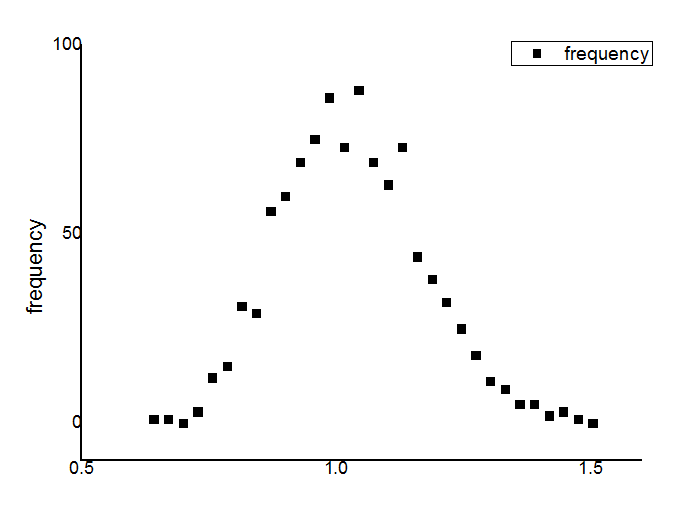
\includegraphics[scale=0.7]{figure2-03}
    \caption{Reconstructed $\beta$ from 1000 thousand runs each with 1000 time steps. Statistics is $\beta=1.009\pm0.017$.}
    \label{fig:1}
\end{figure}

\begin{figure}
    \centering
    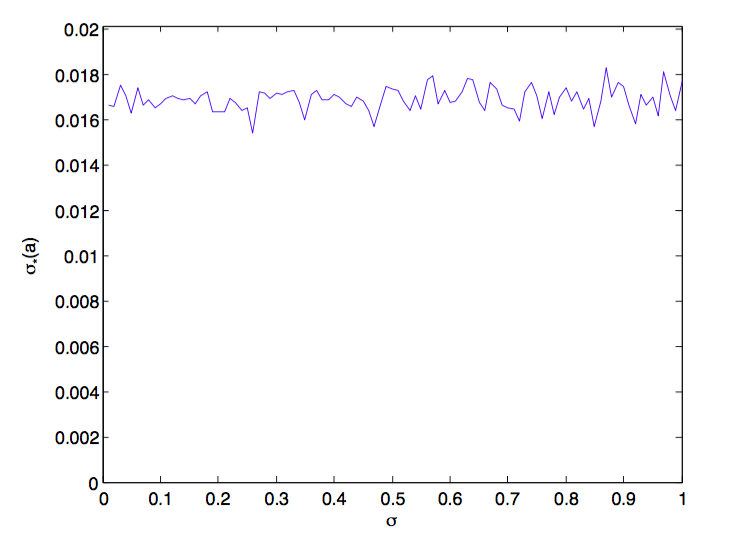
\includegraphics[scale=0.65]{Fig2-04}
    \caption{$\Delta \beta$ versus the level of the noise $\sigma$. No correlation is observed.}
    \label{fig:2}
\end{figure}

\begin{figure}
    \centering
    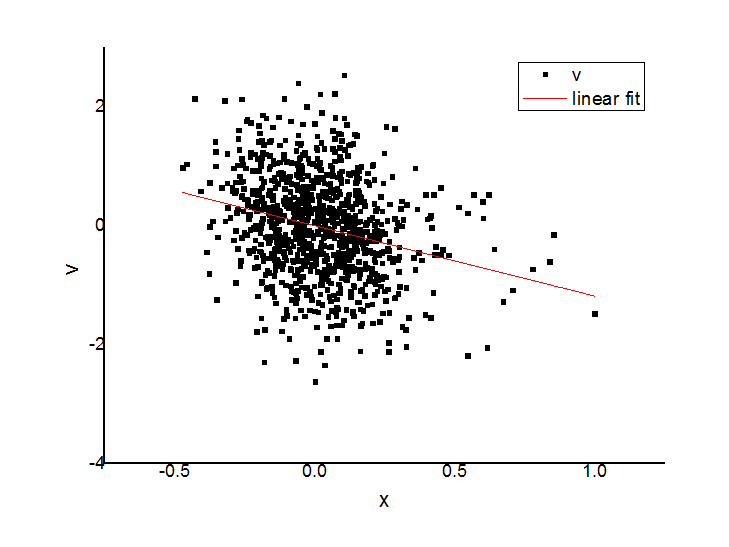
\includegraphics[scale=0.75]{figure2-02}
    \caption{Scatter of $v$ versus $y$ with $\sigma=0.5$.}
    \label{fig:3}
\end{figure}

\begin{figure}
    \centering
    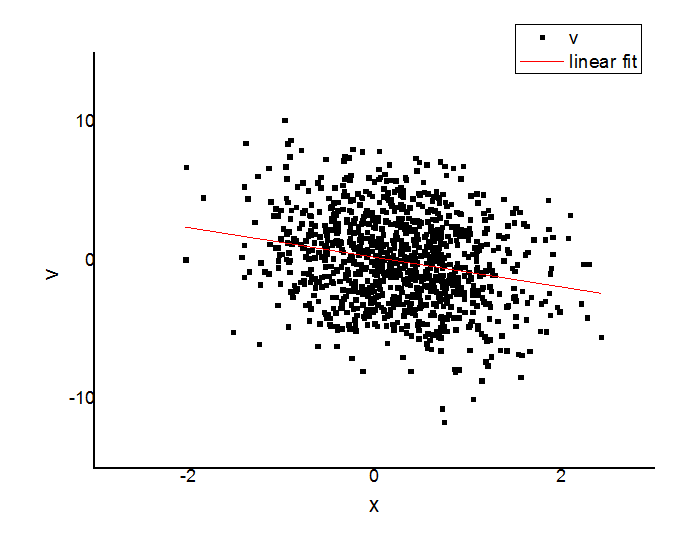
\includegraphics[scale=0.75]{figure2-01}
    \caption{Scatter of $v$ versus $y$ with $\sigma=1$.}
    \label{fig:4}
\end{figure}

\begin{figure}
    \centering
    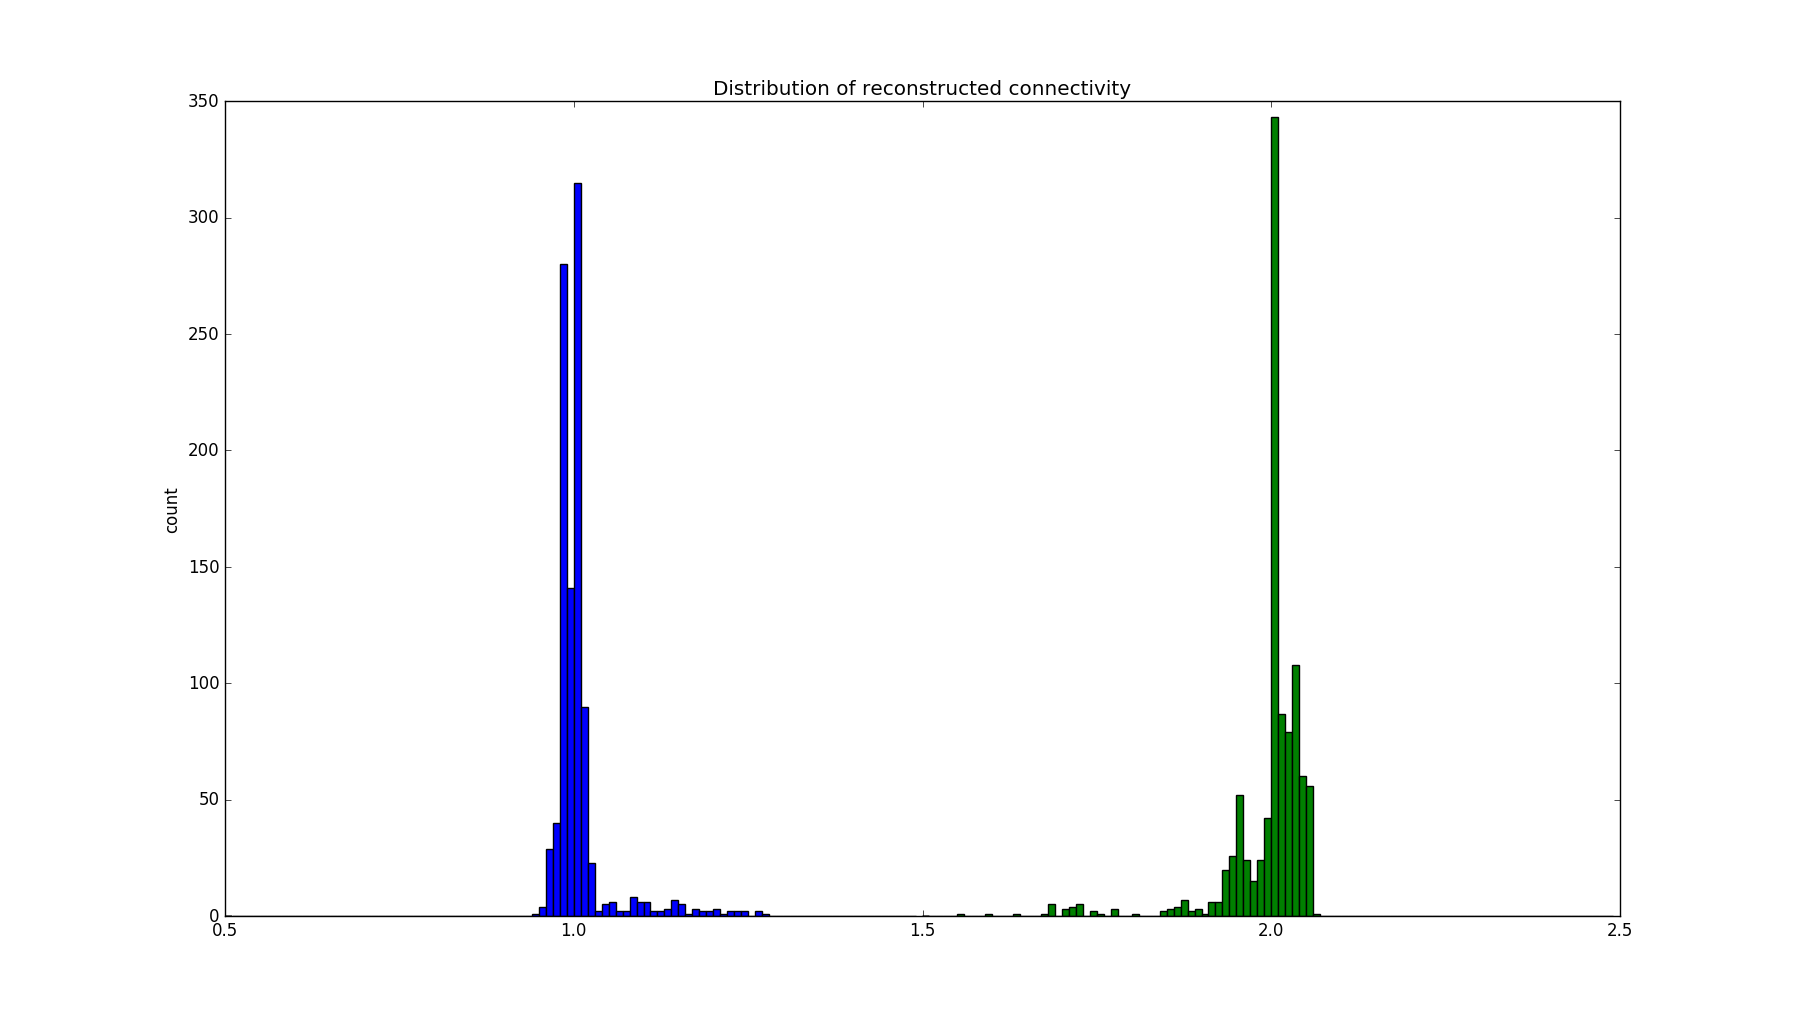
\includegraphics[scale=0.42]{2linear}
    \caption{Distribution of $\beta_1=1.035 \pm 0.041$ and $\beta_2=1.982 \pm 0.065$. To compare, the original connecitivity is $\alpha_1=1$ and $\alpha_2=2$.}
    \label{fig:5}
\end{figure}

\begin{figure}
    \centering
    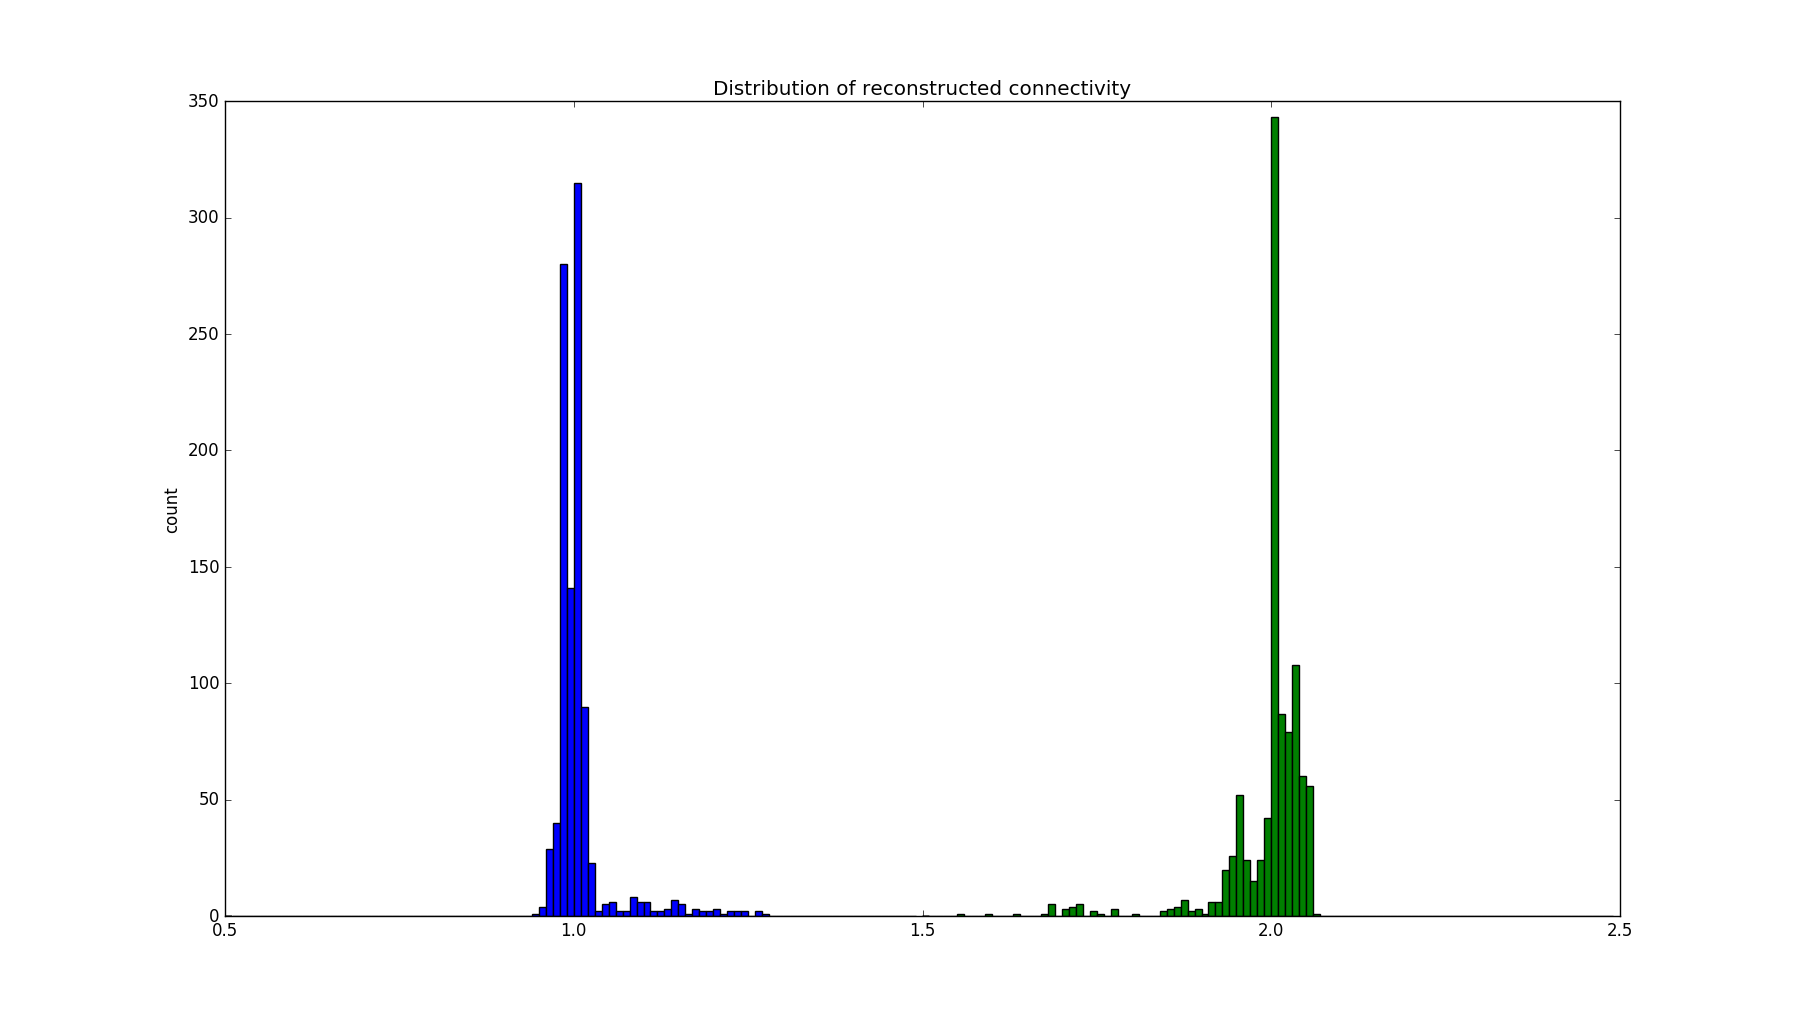
\includegraphics[scale=0.42]{2linear}
    \caption{Distribution of $\beta_1=1.011 \pm 0.038$ and $\beta_2=2.015 \pm 0.017$ for the sinusoidal coupling. To compare, the original connectivity is $\alpha_1=1$ and $\alpha_2=2$.}
    \label{fig:6}
\end{figure}

\end{document}
